% ------------------------------------------------------------
% LaTeX Template für die DHBW zum Schnellstart!
% Original: https://github.wdf.sap.corp/vtgermany/LaTeX-Template-DHBW
% ------------------------------------------------------------
% ---- Präambel mit Angaben zum Dokument
% LTeX: enabled=false

\documentclass[
	fontsize=12pt,           % Leitlinien sprechen von Schriftgröße 12.
	paper=A4,
	twoside=false,
	listof=totoc,            % Tabellen- und Abbildungsverzeichnis ins Inhaltsverzeichnis
	bibliography=totoc,      % Literaturverzeichnis ins Inhaltsverzeichnis aufnehmen
	titlepage,               % Titlepage-Umgebung anstatt \maketitle
	headsepline,             % horizontale Linie unter Kolumnentitel
	abstract,              % Überschrift einschalten, Abstract muss in {abstract}-Umgebung stehen
]{scrreprt}                  % Verwendung von KOMA-Report
\usepackage[utf8]{inputenc}  % UTF8 Encoding einschalten
\usepackage[ngerman,american]{babel}  % Neue deutsche Rechtschreibung
% \usepackage[T1]{fontenc}     % Ausgabe von westeuropäischen Zeichen (auch Umlaute)
% \usepackage{fontspec}
\usepackage{microtype}       % Trennung von Wörtern wird besser umgesetzt
\usepackage{lmodern}         % Nicht-gerasterte Schriftarten (bei MikTeX erforderlich)
\usepackage{graphicx}        % Einbinden von Grafiken erlauben
\usepackage{rotating}        % Rotieren von Grafiken ermöglichen
\usepackage{adjustbox}
\usepackage{wrapfig}         % Grafiken fließend im Text
\usepackage{setspace}        % Zeilenabstand \singlespacing, \onehalfspaceing, \doublespacing
\usepackage[
	%showframe,                % Ränder anzeigen lassen
	left=2.7cm, right=2.5cm,
	top=2.5cm,  bottom=2.5cm,
	includeheadfoot,
	a4paper
]{geometry}                      % Seitenlayout einstellen
\usepackage{scrlayer-scrpage}    % Gestaltung von Fuß- und Kopfzeilen
\usepackage[printonlyused]{acronym}             % Abkürzungen, Abkürzungsverzeichnis
\usepackage{titletoc}            % Anpassungen am Inhaltsverzeichnis
\contentsmargin{0.75cm}          % Abstand im Inhaltsverzeichnis zw. Punkt und Seitenzahl
\usepackage[                     % Klickbare Links (enth. auch "nameref", "url" Package)
  hidelinks,                     % Blende die "URL Boxen" aus.
  breaklinks=true                % Breche zu lange URLs am Zeilenende um
]{hyperref}
\usepackage[hypcap=true]{caption}% Anker Anpassung für Referenzen
\urlstyle{same}                  % Aktuelle Schrift auch für URLs
% Anpassung von autoref für Gleichungen (ergänzt runde Klammern) und Algorithm.
% Anstatt "Listing" kann auch z.B. "Code-Ausschnitt" verwendet werden. Dies sollte
% jedoch synchron gehalten werden mit \lstlistingname (siehe weiter unten).
\addto\extrasngerman{%
	\def\equationautorefname~#1\null{Gleichung~(#1)\null}
	\def\lstnumberautorefname{Zeile}
	\def\lstlistingautorefname{Listing}
	\def\algorithmautorefname{Algorithmus}
	% Damit einheitlich "Abschnitt 1.2[.3]" verwendet wird und nicht "Unterabschnitt 1.2.3"
	% \def\subsectionautorefname{Abschnitt}
}

% ---- Abstand verkleinern von der Überschrift 
\renewcommand*{\chapterheadstartvskip}{\vspace*{.5\baselineskip}}

% Hierdurch werden Schusterjungen und Hurenkinder vermieden, d.h. einzelne Wörter
% auf der nächsten Seite oder in einer einzigen Zeile.
% LaTeX kann diese dennoch erzeugen, falls das Layout ansonsten nicht umsetzbar ist.
% Diese Werte sind aber gute Startwerte.
\widowpenalty10000
\clubpenalty10000

% ---- Für das Quellenverzeichnis
\usepackage[
	backend = biber,                % Verweis auf biber
	language = auto,
	style = numeric,                % Nummerierung der Quellen mit Zahlen
	sorting = none,                 % none = Sortierung nach der Erscheinung im Dokument
	sortcites = true,               % Sortiert die Quellen innerhalb eines cite-Befehls
	block = space,                  % Extra Leerzeichen zwischen Blocks
	hyperref = true,                % Links sind klickbar auch in der Quelle
	%backref = true,                % Referenz, auf den Text an die zitierte Stelle
	bibencoding = auto,
	giveninits = true,              % Vornamen werden abgekürzt
	doi=false,                      % DOI nicht anzeigen
	isbn=false,                     % ISBN nicht anzeigen
    alldates=short                  % Datum immer als DD.MM.YYYY anzeigen
]{biblatex}
\addbibresource{library.bib}
\setcounter{biburlnumpenalty}{3000}     % Umbruchgrenze für Zahlen
\setcounter{biburlucpenalty}{6000}      % Umbruchgrenze für Großbuchstaben
\setcounter{biburllcpenalty}{9000}      % Umbruchgrenze für Kleinbuchstaben
\DeclareNameAlias{default}{family-given}  % Nachname vor dem Vornamen
\AtBeginBibliography{\renewcommand{\multinamedelim}{\addslash\space
}\renewcommand{\finalnamedelim}{\multinamedelim}}  % Schrägstrich zwischen den Autorennamen
\DefineBibliographyStrings{german}{
  urlseen = {Einsichtnahme:},                      % Ändern des Titels von "besucht am"
}
\usepackage[babel,german=quotes]{csquotes}         % Deutsche Anführungszeichen + Zitate


% ---- Für Mathevorlage
\usepackage{amsmath}    % Erweiterung vom Mathe-Satz
\usepackage{amssymb}    % Lädt amsfonts und weitere Symbole
\usepackage{MnSymbol}   % Für Symbole, die in amssymb nicht enthalten sind.

% ---- Für chemische Formeln
\usepackage{mhchem}

% ---- Für Quellcodevorlage
\usepackage{scrhack}                    % Hack zur Verw. von listings in KOMA-Script
\usepackage{listings}                   % Darstellung von Quellcode
\usepackage{xcolor}                     % Einfache Verwendung von Farben
% -- Eigene Farben für den Quellcode
\definecolor{JavaLila}{rgb}{0.4,0.1,0.4}
\definecolor{JavaGruen}{rgb}{0.3,0.5,0.4}
\definecolor{JavaBlau}{rgb}{0.0,0.0,1.0}
\definecolor{ABAPKeywordsBlue}{HTML}{6000ff}
\definecolor{ABAPCommentGrey}{HTML}{808080}
\definecolor{ABAPStringGreen}{HTML}{4da619}
\definecolor{PyKeywordsBlue}{HTML}{0000AC}
\definecolor{PyCommentGrey}{HTML}{808080}
\definecolor{PyStringGreen}{HTML}{008080}
% -- Farben für ABAP CDS
\definecolor{CDSString}{HTML}{FF8C00}
\definecolor{CDSKeywords}{HTML}{6000ff}
\definecolor{CDSAnnotation}{HTML}{00BFFF}
\definecolor{CDSComment}{HTML}{808080}
\definecolor{CDSFunc}{HTML}{FF0000}

% -- Default Listing-Styles

\lstset{
	% Das Paket "listings" kann kein UTF-8. Deswegen werden hier 
	% die häufigsten Zeichen definiert (ä,ö,ü,...)
	literate=%
		{á}{{\'a}}1 {é}{{\'e}}1 {í}{{\'i}}1 {ó}{{\'o}}1 {ú}{{\'u}}1
		{Á}{{\'A}}1 {É}{{\'E}}1 {Í}{{\'I}}1 {Ó}{{\'O}}1 {Ú}{{\'U}}1
		{à}{{\`a}}1 {è}{{\`e}}1 {ì}{{\`i}}1 {ò}{{\`o}}1 {ù}{{\`u}}1
		{À}{{\`A}}1 {È}{{\'E}}1 {Ì}{{\`I}}1 {Ò}{{\`O}}1 {Ù}{{\`U}}1
		{ä}{{\"a}}1 {ë}{{\"e}}1 {ï}{{\"i}}1 {ö}{{\"o}}1 {ü}{{\"u}}1
		{Ä}{{\"A}}1 {Ë}{{\"E}}1 {Ï}{{\"I}}1 {Ö}{{\"O}}1 {Ü}{{\"U}}1
		{â}{{\^a}}1 {ê}{{\^e}}1 {î}{{\^i}}1 {ô}{{\^o}}1 {û}{{\^u}}1
		{Â}{{\^A}}1 {Ê}{{\^E}}1 {Î}{{\^I}}1 {Ô}{{\^O}}1 {Û}{{\^U}}1
		{œ}{{\oe}}1 {Œ}{{\OE}}1 {æ}{{\ae}}1 {Æ}{{\AE}}1 {ß}{{\ss}}1
		{ű}{{\H{u}}}1 {Ű}{{\H{U}}}1 {ő}{{\H{o}}}1 {Ő}{{\H{O}}}1
		{ç}{{\c c}}1 {Ç}{{\c C}}1 {ø}{{\o}}1 {å}{{\r a}}1 {Å}{{\r A}}1
		{€}{{\euro}}1 {£}{{\pounds}}1 {«}{{\guillemotleft}}1
		{»}{{\guillemotright}}1 {ñ}{{\~n}}1 {Ñ}{{\~N}}1 {¿}{{?`}}1,
	breaklines=true,        % Breche lange Zeilen um 
	breakatwhitespace=true, % Wenn möglich, bei Leerzeichen umbrechen
	% Symbol für Zeilenumbruch einfügen
	prebreak=\raisebox{0ex}[0ex][0ex]{\ensuremath{\rhookswarrow}},
	postbreak=\raisebox{0ex}[0ex][0ex]{\ensuremath{\rcurvearrowse\space}},
	tabsize=4,                                 % Setze die Breite eines Tabs
	basicstyle=\ttfamily\small,                % Grundsätzlicher Schriftstyle
	columns=fixed,                             % Besseres Schriftbild
	numbers=left,                              % Nummerierung der Zeilen
	%frame=single,                             % Umrandung des Codes
	showstringspaces=false,                    % Keine Leerzeichen hervorheben
	keywordstyle=\color{blue},
	ndkeywordstyle=\bfseries\color{darkgray},
	identifierstyle=\color{black},
	commentstyle=\itshape\color{JavaGruen},   % Kommentare in eigener Farbe
	stringstyle=\color{JavaBlau},             % Strings in eigener Farbe,
	captionpos=b,                             % Bild*unter*schrift
	xleftmargin=5.0ex
}

% ---- Eigener JAVA-Style für den Quellcode
\renewcommand{\ttdefault}{pcr}               % Schriftart, welche auch fett beinhaltet
\lstdefinestyle{EigenerJavaStyle}{
	language=Java,                             % Syntax Highlighting für Java
	%frame=single,                             % Umrandung des Codes
	keywordstyle=\bfseries\color{JavaLila},    % Keywords in eigener Farbe und fett
	commentstyle=\itshape\color{JavaGruen},    % Kommentare in eigener Farbe und italic
	stringstyle=\color{JavaBlau}               % Strings in eigener Farbe
}

% ---- Eigener ABAP-Style für den Quellcode
\renewcommand{\ttdefault}{pcr}
\lstdefinestyle{EigenerABAPStyle}{
	language=[R/3 6.10]ABAP,
	morestring=[b]\|,                          % Für Pipe-Strings
	morestring=[b]\`,                          % für Backtick-Strings
	keywordstyle=\bfseries\color{ABAPKeywordsBlue},
	commentstyle=\itshape\color{ABAPCommentGrey},
	stringstyle=\color{ABAPStringGreen},
	tabsize=2,
	morekeywords={
		types,
		@data,
		as,
		lower,
		start,
		selection,
		order,
		by,
		inner,
		join,
		key,
		end,
		cast
	}
}

% ---- Eigener Python-Style für den Quellcode
\renewcommand{\ttdefault}{pcr}
\lstdefinestyle{EigenerPythonStyle}{
	language=Python,
	columns=flexible,
	keywordstyle=\bfseries\color{PyKeywordsBlue},
	commentstyle=\itshape\color{PyCommentGrey},
	stringstyle=\color{PyStringGreen}
}

%----- ABAP-CDS-View language
\lstdefinelanguage{ABAPCDS}{
	sensitive=false,
	%Keywords
	morekeywords={define,
		view,
		as,
		select,
		from,
		inner,
		join,
		on,
		key,
		case,
		when,
		then,
		else,
		end,
		true,
		false,
		cast,
		where,
		and,
		distinct,
		group,
		by,
		having,
		min,
		sum,
		max,
		count,
		avg
	},
	%Methoden
	morekeywords=[2]{
		div,
		currency\_conversion,
		dats\_days\_between,
		concat\_with\_space,
		dats\_add_days,
		dats\_is\_valid,
		dats\_add\_months,
		unit\_conversion,
		division,
		mod,
		abs,
		floor,
		ceil,
		round,
		concat,
		replace,
		substring,
		left,
		right,
		length
	},
	morecomment=[s][\color{CDSAnnotation}]{@}{:},
	morecomment=[l][\itshape\color{CDSComment}]{//},
	morecomment=[s][\itshape\color{CDSComment}]{/*}{*/},
	morestring=[b][\color{CDSString}]',
	keywordstyle=\bfseries\color{CDSKeywords},
	keywordstyle=[2]\color{CDSFunc}
}

  % Weitere Details sind ausgelagert

\usepackage{algorithm}                  % Für Algorithmen-Umgebung (ähnlich wie lstlistings Umgebung)
\usepackage{algpseudocode}              % Für Pseudocode. Füge "[noend]" hinzu, wenn du kein "endif",
                                        % etc. haben willst.

\makeatletter                           % Sorgt dafür, dass man @ in Namen verwenden kann.
                                        % Ansonsten gibt es in der nächsten Zeile einen Compilefehler.
\renewcommand{\ALG@name}{Algorithmus}   % Umbenennen von "Algorithm" im Header der Listings.
\makeatother                            % Zeichen wieder zurücksetzen
\renewcommand{\lstlistingname}{Listing} % Erlaubt das Umbenennen von "Listing" in anderen Titel.

% ---- Tabellen
\usepackage{booktabs}  % Für schönere Tabellen. Enthält neue Befehle wie \midrule
\usepackage{multirow}  % Mehrzeilige Tabellen
\usepackage{siunitx}   % Für SI Einheiten und das Ausrichten Nachkommastellen
\sisetup{locale=DE, range-phrase={~bis~}, output-decimal-marker={,}} % Damit ein Komma und kein Punkt verwendet wird.
\usepackage{xfrac} % Für siunitx Option "fraction-function=\sfrac"

% ---- Für Definitionsboxen in der Einleitung
\usepackage{amsthm}                     % Liefert die Grundlagen für Theoreme
\usepackage[framemethod=tikz]{mdframed} % Boxen für die Umrandung
% ---- Definition für Highlight Boxen

% ---- Grundsätzliche Definition zum Style
\newtheoremstyle{defi}
  {\topsep}         % Abstand oben
  {\topsep}         % Abstand unten
  {\normalfont}     % Schrift des Bodys
  {0pt}             % Einschub der ersten Zeile
  {\bfseries}       % Darstellung von der Schrift in der Überschrift
  {:}               % Trennzeichen zwischen Überschrift und Body
  {.5em}            % Abstand nach dem Trennzeichen zum Body Text
  {\thmname{#3}}    % Name in eckigen Klammern
\theoremstyle{defi}

% ------ Definition zum Strich vor eines Texts
\newmdtheoremenv[
  hidealllines = true,       % Rahmen komplett ausblenden
  leftline = true,           % Linie links einschalten
  innertopmargin = 0pt,      % Abstand oben
  innerbottommargin = 4pt,   % Abstand unten
  innerrightmargin = 0pt,    % Abstand rechts
  linewidth = 3pt,           % Linienbreite
  linecolor = gray!40,       % Linienfarbe
]{defStrich}{Definition}     % Name der des formats "defStrich"

% ------ Definition zum Eck-Kasten um einen Text
\newmdtheoremenv[
  hidealllines = true,
  innertopmargin = 6pt,
  linecolor = gray!40,
  singleextra={              % Eck-Markierungen für die Definition
    \draw[line width=3pt,gray!50,line cap=rect] (O|-P) -- +(1cm,0pt);
    \draw[line width=3pt,gray!50,line cap=rect] (O|-P) -- +(0pt,-1cm);
    \draw[line width=3pt,gray!50,line cap=rect] (O-|P) -- +(-1cm,0pt);
    \draw[line width=3pt,gray!50,line cap=rect] (O-|P) -- +(0pt,1cm);
  }
]{defEckKasten}{Definition}  % Name der des formats "defEckKasten"  % Weitere Details sind ausgelagert

% ---- Für Todo Notes
\usepackage{todonotes}
\setlength {\marginparwidth }{2cm}      % Abstand für Todo Notizen

\lstdefinelanguage{JavaScript}{
  morekeywords=[1]{break, case, catch, continue, debugger, default, delete, do, else, finally, for, function, if, in, instanceof, new, return, switch, this, throw, try, typeof, var, void, while, with, require, then, const},
  morecomment=[l]{//},
  morecomment=[s]{/*}{*/},
  morestring=[b]{'},
  morestring=[b]{"},
  morestring=[b]{`},
%   alsoletter={\\'},
  stringstyle=\color[rgb]{0.3,0.5,0.4},
  sensitive=true
}

\lstdefinelanguage{Docker}{
	% Keywords as defined in the language grammar
	morekeywords=[1]{%
	  FROM,RUN,COPY,WORKDIR,LABEL,USER,ENTRYPOINT,EXPOSE,CMD},
	% Built-in functions
	morekeywords=[2]{},
	% Pre-declared types
	morekeywords=[3]{},
	% Constants and zero value
	morekeywords=[4]{},
	% Strings : "foo", 'bar', `baz`
	morestring=[b]{"},
	morestring=[b]{'},
	morestring=[b]{`},
	% Comments : /* cpmment */ and // comment
	comment=[l]{\#},
	morecomment=[s]{/*}{*/},
	stringstyle=\color[rgb]{0.3,0.5,0.4},
	% Options
	sensitive=true
}

\lstdefinelanguage{Golang}%
  {morekeywords=[1]{package,import,func,type,struct,return,defer,panic,%
     recover,select,var,const,iota,},%
   morekeywords=[2]{string,uint,uint8,uint16,uint32,uint64,int,int8,int16,%
     int32,int64,bool,float32,float64,complex64,complex128,byte,rune,uintptr,%
     error,interface},%
   morekeywords=[3]{map,slice,make,new,nil,len,cap,copy,close,true,false,%
     delete,append,real,imag,complex,chan,},%
   morekeywords=[4]{for,break,continue,range,go,goto,switch,case,fallthrough,if,%
     else,default,},%
   morekeywords=[5]{Println,Printf,Error,Print,},%
   sensitive=true,%
   morecomment=[l]{//},%
   morecomment=[s]{/*}{*/},%
   morestring=[b]',%
   morestring=[b]",%
   morestring=[s]{`}{`},%
   tabsize = 2,%
}

\usepackage{xurl}

% ---- Elektronische Version oder Gedruckte Version?
% ---- Unterschied: Die elektronische Version enthält keinen Platzhalter für die Unterschrift
\usepackage{ifthen}
\newboolean{e-Abgabe}
\setboolean{e-Abgabe}{false}    % false=gedruckte Fassung

% ---- Persönlichen Daten:
\newcommand{\titel}{Redesigning and Implementing the Bootstrap of Large Scale Kubernetes Enterprise Infrastructure through Automated Self Contained CLI}
\newcommand{\titelheader}{Bootstrapping Kubernetes Infrastructure} % TOOD: is this even needed?
\newcommand{\arbeit}{Project 2b (T3\_2000)}
\newcommand{\studiengang}{Computer Science (Informatik)}
\newcommand{\studienjahr}{2020}
\newcommand{\autor}{Yannik Schiebelhut}
\newcommand{\autorReverse}{Schiebelhut, Yannik}
\newcommand{\verfassungsort}{Karlsruhe}
\newcommand{\matrikelnr}{3354235}
\newcommand{\kurs}{TINF20B1}
\newcommand{\bearbeitungsmonat}{September 2022}
\newcommand{\abgabe}{September 19, 2022}
\newcommand{\bearbeitungszeitraum}{July 4, 2022 - September 19, 2022}
\newcommand{\firmaName}{SAP SE}
\newcommand{\firmaStrasse}{Dietmar-Hopp-Allee 16}
\newcommand{\firmaPlz}{69190 Walldorf, Deutschland}
\newcommand{\betreuerFirma}{Samed Guener} % TODO: doch Jan einsetzen? TODO: Mit Umlaut?
\newcommand{\betreuerDhbw}{Prof. Dr. Johannes Freudenmann}

% ---- Metainformation für das PDF Dokument
\hypersetup{
	pdftitle    = {\titel},
	pdfsubject  = {\arbeit},
	pdfauthor   = {\autor},
	%pdfkeywords = {Keywords angeben},
	pdfcreator  = {LaTeX},
	%pdfproducer = {in der Regel pdfTeX}
}

% ---- Definition der Kopf- und Fußzeilen
\clearscrheadfoot                               % Löschen von LaTeX Standard
\automark[section]{chapter}                     % Füllen von section und chapter
\renewcommand*{\chaptermarkformat}{}            % Entfernt die Kapitelnummer
\renewcommand*{\sectionmarkformat}{}            % Entfernt die Sectionnummer
% Angaben [für "plain"]{für "scrheadings"}
% \ihead[]{\titelheader}                          % Kopfzeile links
\ihead{\ifthenelse{\value{chapter}>0}{\chaptername~\thechapter}{}}
\chead[]{}                                      % Kopfzeile mitte
% \ohead[]{\rightmark}                            % Kopfzeile rechts
\ohead{\ifthenelse{\value{chapter}>0}{\headmark}{}}
\ifoot[]{}                                      % Fußzeile links
\cfoot*{\sffamily\pagemark}                     % Fußzeile mitte
\ofoot[]{}                                      % Fußzeile rechts
\KOMAoptions{
   headsepline = 0.2pt,                         % Liniendicke Kopfzeile
   footsepline = false                          % Liniendicke Fußzeile
}

% ---- Hilfreiches
\newcommand{\zB}{z.\,B. }   % "z.B." mit kleinem Leeraum dazwischen (ohne wäre nicht korrekt)
\newcommand{\dash}{d.\,h. }
\newcommand{\Dash}{D.\,h. }

\newcommand{\code}[1]{\texttt{#1}} % Ist einfacher zu schreiben als ständig \texttt und erlaubt
                                   % Änderungen im Nachhinein, wenn man z.B. Inline-Code anders stylen möchte.

% ---- Silbentrennung (falls LaTeX defaults falsch / nicht gewünscht sind)
\hyphenation{HANA}         % anstatt HA-NA
\hyphenation{Graph-Script} % anstatt GraphS-cript

% ---- Beginn des Dokuments
\begin{document}
\setlength{\parindent}{0pt}              % Keine Paragraphen Einrückung.
                                         % Dafür haben wir den Abstand zwischen den Paragraphen.
\setcounter{secnumdepth}{2}              % Nummerierungstiefe fürs Inhaltsverzeichnis
\setcounter{tocdepth}{1}                 % Tiefe des Inhaltsverzeichnisses. Ggf. so anpassen,
                                         % dass das Verzeichnis auf eine Seite passt.
\sffamily                                % Serifenlose Schrift verwenden.

% ---- Vorspann
% ------ Titelseite
\singlespacing
\begin{otherlanguage}{ngerman}
    \thispagestyle{empty}
\begin{titlepage}
\enlargethispage{4cm}

\begin{figure}           % Logo vom Ausbildungsbetrieb und der DHBW
	% \vspace*{-5mm} % Sollte dein Titel zu lang werden, kannst du mit diesem "Hack" 
	%                  den Inhalt der Seite nach oben schieben.
	\begin{minipage}{0.49\textwidth}
		\flushleft
		
\includegraphics[height=2.5cm]{Bilder/Logos/Logo_SAP.pdf} 
	\end{minipage}
	\hfill
	\begin{minipage}{0.49\textwidth}
		\flushright
		
\includegraphics[height=2.5cm]{Bilder/Logos/Logo_DHBW.pdf} 
	\end{minipage}
\end{figure} 
\vspace*{0.1cm}

\begin{center}
	\huge{\textbf{\titel}}\\[1.5cm]
	\Large{\textbf{\arbeit}}\\[0.5cm]
	\normalsize{in the context of the examination for the\\[1ex] \textbf{Bachelor of Science (B.Sc.)}}\\[0.5cm]
	\Large{in \studiengang}\\[1ex]
	\normalsize{at the Cooperative State University Baden-Württemberg Karlsruhe}\\[1cm]
	\normalsize{by}\\[1ex] \Large{\textbf{\autor}} \\[1cm]
\end{center}

\begin{center}
	\vfill
	\begin{tabular}{ll}
		Submission Date:                               & \abgabe \\[0.2cm]
		Processing period:                             & \bearbeitungszeitraum \\[0.2cm]
		Matriculation number, Course:                  & \matrikelnr , \kurs \\[0.2cm]
		Training institution:                          & \firmaName \\
		                                               & \firmaStrasse \\
		                                               & \firmaPlz \\[0.2cm]
		Supervisor of the training institution:        & \betreuerFirma \\[0.2cm]
		Appraiser of the Cooperative State University: & \betreuerDhbw \\[2cm]
	\end{tabular} 
\end{center}
\end{titlepage}
  % Titelseite
\end{otherlanguage}
\newcounter{savepage}
\pagenumbering{Roman}                    % Römische Seitenzahlen
\onehalfspacing

\begin{otherlanguage}{ngerman}
    % ------ Erklärung, Sperrvermerk, Abstact
    \chapter*{Eidesstattliche Erklärung}
Ich versichere hiermit, dass ich meine \arbeit{} mit dem Thema:
\begin{quote}
	\textit{\titel}
\end{quote} 
gemäß § 5 der \enquote{Studien- und Prüfungsordnung DHBW Technik} vom 29. September 2017 selbstständig verfasst und keine anderen als die angegebenen Quellen und Hilfsmittel benutzt habe. Die Arbeit wurde bisher keiner anderen Prüfungsbehörde vorgelegt und auch nicht veröffentlicht.

\vspace{0.25cm}

Ich versichere zudem, dass die eingereichte elektronische Fassung mit der gedruckten Fassung übereinstimmt.

\vspace{1cm}

\verfassungsort, den \today \\[0.5cm]
\ifthenelse{\boolean{e-Abgabe}}
	{\underline{Gez. \autor}}
	{\makebox[6cm]{\hrulefill}}\\ 
\autorReverse

    \chapter*{Sperrvermerk}
Die nachfolgende Arbeit enthält vertrauliche Daten der:
\begin{quote}
	\firmaName \\
	\firmaStrasse \\
	\firmaPlz
\end{quote}

\vspace{0.5cm}

Der Inhalt dieser Arbeit darf weder als Ganzes noch in Auszügen Personen außerhalb des Prüfungsprozesses und des Evaluationsverfahrens zugänglich gemacht werden, sofern keine anderslautende Genehmigung vom Dualen Partner vorliegt.

    \renewcommand{\abstractname}{Abstract} % Veränderter Name für das Abstract
\begin{abstract}
\begin{addmargin}[1.5cm]{1.5cm}        % Erhöhte Ränder, für Abstract Look
\thispagestyle{plain}                  % Seitenzahl auf der Abstract Seite

\begin{center}
\small\textit{- Deutsch -}             % Angabe der Sprache für das Abstract
\end{center}

\vspace{0.25cm}

% LTeX: language=de-DE

Platzhalter

\end{addmargin}
\end{abstract}
    \renewcommand{\abstractname}{Abstract} % Veränderter Name für das Abstract
\begin{abstract}
\begin{addmargin}[1.5cm]{1.5cm}        % Erhöhte Ränder, für Abstract Look
\thispagestyle{plain}                  % Seitenzahl auf der Abstract Seite

\begin{center}
\small\textit{- English -}             % Angabe der Sprache für das Abstract
\end{center}

\vspace{0.25cm}

% LTeX: language=en-US

In order to raise cross company processes to a new level SAP is working on the development of \acl*{ccwf}.
The shared process data is to be imported into \emph{Signavio Process Intelligence} to be analyzed with process mining and to be presented in \aclp*{kpi}.
Since \acl*{ccwf} uses the \emph{SAP Blockchain} to store data the preparation of the data for analysis within Signavio is a challenge.

\vspace{0.25cm}

In the context of this report, these difficulties will first be discussed.
It then deals with the conceptual design of a data integration process.
For this purpose, on the one hand, it is discussed where the conversion of the data from \acl*{ccwf} into the target format should be carried out.
On the other hand, different transport routes are discussed, through which the processed data should be made available in Signavio Process Intelligence.
Based on the developed concept, a prototype of the data integration is implemented.

\end{addmargin}
\end{abstract}
\end{otherlanguage}

% ------ Inhaltsverzeichnis
\singlespacing
\tableofcontents

% ------ Verzeichnisse
\renewcommand*{\chapterpagestyle}{plain}
\pagestyle{plain}
% \chapter*{Formelverzeichnis}
\addcontentsline{toc}{chapter}{Formelverzeichnis} % Hinzufügen zum Inhaltsverzeichnis 

% Definition des neuen Befehls für das Einfügen der Abkürzung der Einheit
\newcommand{\acrounit}[1]{
  \acroextra{\makebox[18mm][l]{\si[per-mode=fraction,fraction-function=\sfrac]{#1}}}
}
\begin{acronym}[dmin] % längstes Kürzel wird verw. für den Abstand zw. Kürzel u. Text

	% Alphabetisch selbst sortieren - nicht verwendete Formeln rausnehmen!
	% Allgemein: \acro{KÜRZEL}[ABKÜRZUNG]{\acrounit{SI-EINHEIT}BESCHREIBUNG}

	\acro{A}[\ensuremath{A}]{\acrounit{mm^2}Fläche}	
	\acro{D}[\ensuremath{D}]{\acrounit{mm}Werkstückdurchmesser}	
	\acro{dmin}[\ensuremath{d\textsubscript{min}}]{\acrounit{mm}kleinster Schaftdurchmesser}	
	\acro{L1}[\ensuremath{L\textsubscript{1}}]{\acrounit{mm}Länge des Werkstückes Nr. 1}	
	\acro{Fwinkel}[]{\acrounit{Grad}Freiwinkel}	
	\acro{Kwinkel}[]{\acrounit{Grad}Keilwinkel}

\end{acronym}

\chapter*{List of Abbreviations}
\addcontentsline{toc}{chapter}{List of Abbreviations} % Hinzufügen zum Inhaltsverzeichnis 

\begin{acronym}[BPMN] % längstes Kürzel wird verw. für den Abstand zw. Kürzel u. Text

	% Alphabetisch selbst sortieren - nicht verwendete Kürzel rausnehmen!
	\acro{acl}[ACL]{Access Control List}
	% \acro{AIR}{Adobe Integrated Runtime}
	% \acro{AJAX}{Asynchronous Javascript and XML}
	% \acro{ANSI}{American National Standards Institute}
	\acro{api}[API]{Application Programming Interface}
	% \acro{AR}{Augmented Reality}
	\acro{aws}[AWS]{Amazon Web Services}
	% \acro{BAPI}{Business Application Programming Interface}
	% \acro{BIOS}{Basic Input Output System}
	\acro{bpmn}[BPMN]{Business Process Model and Notation}
	\acro{ccwf}[ccWF]{Cross-Company Workflow}
	% \acro{CDMA}{Code Division Multiple Access}
	\acro{cicd}[CICD]{Continuous Integration and Continuous Delivery}
	\acro{cli}[CLI]{command-line interface}
	\acro{csv}[CSV]{Comma-Separated Values}
	\acro{eks}[EKS]{Elastic Kubernetes Service}
	\acro{erp}[ERP]{Enterprise Resource Planning}
	\acro{hcl}[HCL]{HashiCorp Configuration Language}
	\acro{hs2}[HS2]{High Speed 2}
	\acro{http}[HTTP]{Hypertext Transfer Protocol}
	% \acro{HTTPS}{Hypertext Transfer Protocol Secure}
	\acro{iaas}[IaaS]{Infrastructure as a Service}
	\acro{iac}[IaC]{Infrastructure as Code}
	% \acro{IP}{Internet Protocol}
	% \acro{ISBN}{Internationale Standardbuchnummer}
	% \acrodefplural{ISBN}[ISBNs]{Internationale Standardbuchnummern}
	\acro{json}[JSON]{JavaScript Object Notation}
	\acro{kpi}[KPI]{Key Performance Indicator}
	% \acro{OData}{Open Data Protocol}
	\acro{rest}[REST]{Representational State Transfer}
	\acro{s3}[S3]{Simple Storage Service}
	\acro{saml}[SAML]{Security Assertion Markup Language}
	\acro{sdk}[SDK]{Software Development Kit}
	% \acro{SEO}{Search Engine Optimization}
	\acro{sql}[SQL]{Structured Query Language}
	% \acro{SSH}{Secure Shell}
	% \acro{UEFI}{Unified Extensible Firmware Interface}
	% \acro{URI}{Uniform Resource Identifier}
	\acro{url}[URL]{Uniform Resource Locator}
	% \acro{USB}{Universal Serial Bus}
	\acro{vcs}[VCS]{Version Control System}
	% \acro{VLAN}{Virtual Local Area Network}
	% \acro{WYSISWG}{What You See Is What You Get}
	\acro{xes}[XES]{eXtensible Event Stream}
	% \acro{XSL}{Extensible Stylesheet Language}

\end{acronym}
\listoffigures                          % Erzeugen des Abbildungsverzeichnisses 
% \listoftables                           % Erzeugen des Tabellenverzeichnisses
\renewcommand{\lstlistlistingname}{List of Code Listings}
\lstlistoflistings                      % Erzeugen des Listenverzeichnisses
\setcounter{savepage}{\value{page}}


% ---- Inhalt der Arbeit
\cleardoublepage
\pagenumbering{arabic}                  % Arabische Seitenzahlen für den Hauptteil
\setlength{\parskip}{0.5\baselineskip}  % Abstand zwischen Absätzen
\rmfamily
\renewcommand*{\chapterpagestyle}{scrheadings}
\pagestyle{scrheadings}
\onehalfspacing
% \include{content goes here}
\chapter{Introduction}
\section{Motivation}
Modern enterprise infrastructure for software development often makes use of cloud computing to dynamically adapt infrastructure to the fast-paced world of agile development.
The setup process of one so-called cluster is traditionally done by hand and can easily require multiple days of work to complete.
Obviously, in consequence of the required man-hours, this manual deployment is rather costly and time-consuming.
Also, humans are prune to error.
In a manual task that big, it is very likely for unforeseeable errors to occur.
Finding these mistakes can eventually take additional time.

As a conclusion, it is desired to automate as much of a clusters' deployment process as possible.
There are already various tools available that can be leveraged to perform an automated deployment of a declared cluster infrastructure.
But even these automatization tools require some perquisites to run, like a technical access user with access to the necessary resources and access keys to make use of this user, which still have to be created manually or with the help of bare-bones scripts.
The process of fulfilling these requirements is referred to as bootstrap.

\section{Goal}
Goal of this project is to simplify the bootstrap of a cluster by integrating the necessary functionality into a \ac{cli} which is currently developed by the supervising department.
Also, the usage should be convenient and, beside providing login data for the cloud provider and credential store, minimal user input should be required to perform the bootstrap.
Furthermore, the newly developed \ac{cli} is required to be able to get executed by an automated build server.
The ways of user interaction have to be designed accordingly.

\section{Approach}

\chapter{Fundamentals}
\section{Go}
Go (also known as Golang) is an open source programming language that was started at Google in 2007 and initially launched in 2009.
The language was designed to face engineering challenges at Google with the goal to make it \enquote{easy to build simple, reliable and efficient software}. \cite{pike.2020, golang.github}
By now, the compiled and statically typed language \cite{chris.2021} is widely used, and the way it approaches network concurrency and software engineering has influenced other languages to a noticeable extent. \cite{pike.2020}
Through its structure Go supports programming on various levels of abstraction.
For instance, one can embed Assembler or C code into a Go program or on the other hand combine groups of components into bigger, more complex components to realize abstract design patterns. \cite{Maurer2021}
Nowadays, Go is a popular choice for everything related to DevOps and therefore also for the development of command line tools. \cite{mike.2020}

Go also tries to provide its own, official solutions for common tasks in software development.
When installing Go, it comes packed alongside with a formatter (which shall ensure uniform styling across all programs written in Go) and an included suite for unit testing, just to name a few examples.
Furthermore, Go supports generating documentation based on comments in the source code; much alike JavaDoc.
Go features an extensive standard library which depicts a good starting point for developing your own applications.
In case one wants to include a third party library, this can be done via the \emph{go get} command.
It fetches the necessary resources (usually directly from a \ac{vcs}) and saves the modules as a dependency in the \emph{go.mod} file. \cite{go.tour, go.docs}

% \begin{itemize}
%     \item toolchain (uniform formatter, included test suite, source code based generation of documentation)
%     \item third party modules repo / go get
%     \item extensive standard library
%     \item (cite from golang.org tutorial)
% \end{itemize}

% started in 2007 released in 2009
% open source, compiled, and statically typed programming language (https://www.freecodecamp.org/news/what-is-go-programming-language/)
% face engineering challenges at Google (https://go.dev/solutions/google/)
% goals: make it "easy to build simple, reliable and efficient software" (https://github.com/golang/go)
% by now widely used
% network concurrency and software engineering are influencing other languages (https://go.dev/solutions/google/)
% through its structure go supports programming on various layers of abstraction (cite from book here)
%     supports embedded assembler and c
%     suitable for realizing abstract design patterns

\subsection{Cobra}
Cobra is an open source library for Go.
Its aim is to provide developers with an easy way to create modern \ac{cli} applications.
The cobra library is being used by noticeable projects like the \ac{cli}s for Kubernetes or for GitHub.
The idea behind Cobra's intended command schema is that commands of a well constructed \ac{cli} should read like sentences.
This way, new users that are familiar with \acp{cli} in general quickly feel native because interacting with the \ac{cli} feels more natural.
In this approach, a command represents a certain action that the \ac{cli} can perform.
This action than take arguments and flags to further specify on which objects and in which way the command should take action.
With Cobra, one can also easily create nested subcommands.
This means that a before mentioned command can also be divided into multiple sub-actions to enable detailed handling of complex actions.
Further, benefits of Cobra are, among others, the automated generation of autocompletion for the most common shells as well as the ability to automatically create man pages. \cite{cobra.github, cobra.dev}
The \ac{cli} that the supervising department is currently developing is build upon Cobra.


% \begin{itemize}
% 	\item open source library
%     \item modern cli applications
%     \item "namenhafte" projects like Kubernetes, GitHub CLI
%     \item subcommand-based -> explain
%     \item nested subcommands
%     \item can automatically generate autocomplete
%     \item helps in generating man pages \cite{cobra.github}
% \end{itemize}

\section{Kubernetes}
\label{sec:kubernetes}
Kubernetes (often short: k8s) is an open source solution to ease up and automate management of container based services.
It follows a declarative paradigm.
This means that the user just needs to describe the desired state -- for example through the use of configuration files or via the Kubernetes \ac{cli} -- and Kubernetes determines the steps by itself which are necessary to reach and maintain this state.
Kubernetes also enables users to dynamically scale their applications and services.
This means that the amount of resources, that are dedicated to an application, is adapted during runtime dependent, for example, on the current number of users.
Furthermore, Kubernetes can perform load balancing and redundancy between different instances of the same service.
\cite{Bloß2019, wasistk8s}

One instance of a Kubernetes system is called a cluster.
A Cluster is composed of multiple nodes (which usually are virtual machines or physical servers) which run the actual applications.
An Application runs inside some kind of container, internally called Pod.
The interaction with a cluster is managed by the so-called \emph{Kubernetes Master}.
It is a central controlling unit.
The user actually never interacts with the nodes themselves directly.
\cite{k8skonzepte}

\section{Gardener}
Even though there are tools that help with creating and updating single Kubernetes clusters, it is rather hard to manage many clusters.
This is where Gardener comes into play.
It is a Kubernetes native extension that manages Kubernetes clusters as a service, packing the performance to manage up to thousands of clusters.
One key concept that is applied is so-called self-hosting.
This means that Kubernetes components are run inside of Kubernetes clusters, and is done because Kubernetes is the go-to way to easily manage software in the cloud. \cite{gardener.architecture, gardener.blog1, gardener.blog2, gardener.cloud}

Gardener's architecture is constructed much like Kubernetes itself although not individual Pods are managed but entire clusters.
The root of all is the so-called \emph{Garden Cluster}.
It is the main interface for the Gardener administrator and hosts, among others, the Garden Cluster control plane, the Gardener dashboard, the Gardener \ac{api} server, the Gardener controller manager, and the Gardener scheduler.
Then there are two other types of clusters, \emph{Seed Clusters} and \emph{Shoot Clusters}.
One Seed Clusters manages the control planes (thus \ac{api} server, scheduler, controller manager, machine controller etc.) of its Shoot Clusters.
There is at least one Seed Cluster per \ac{iaas} provider and region.
The Shoot Clusters control planes are deployed as Pods inside the Seed Cluster, can therefore be created with standard Kubernetes deployment and support rolling updates.
Shoot Clusters only contain worker nodes and are the Kubernetes Clusters that actually become available to the end-user and can be ordered in a declarative way.
The clusters created by Gardener are vanilla Kubernetes clusters independent of the underlying cloud provider. \cite{gardener.blog2, wasistgardener}
(More details of the described architecture can be seen in \autoref{fig:gardener-architecture}.)

\begin{figure}[H]
    \centering
    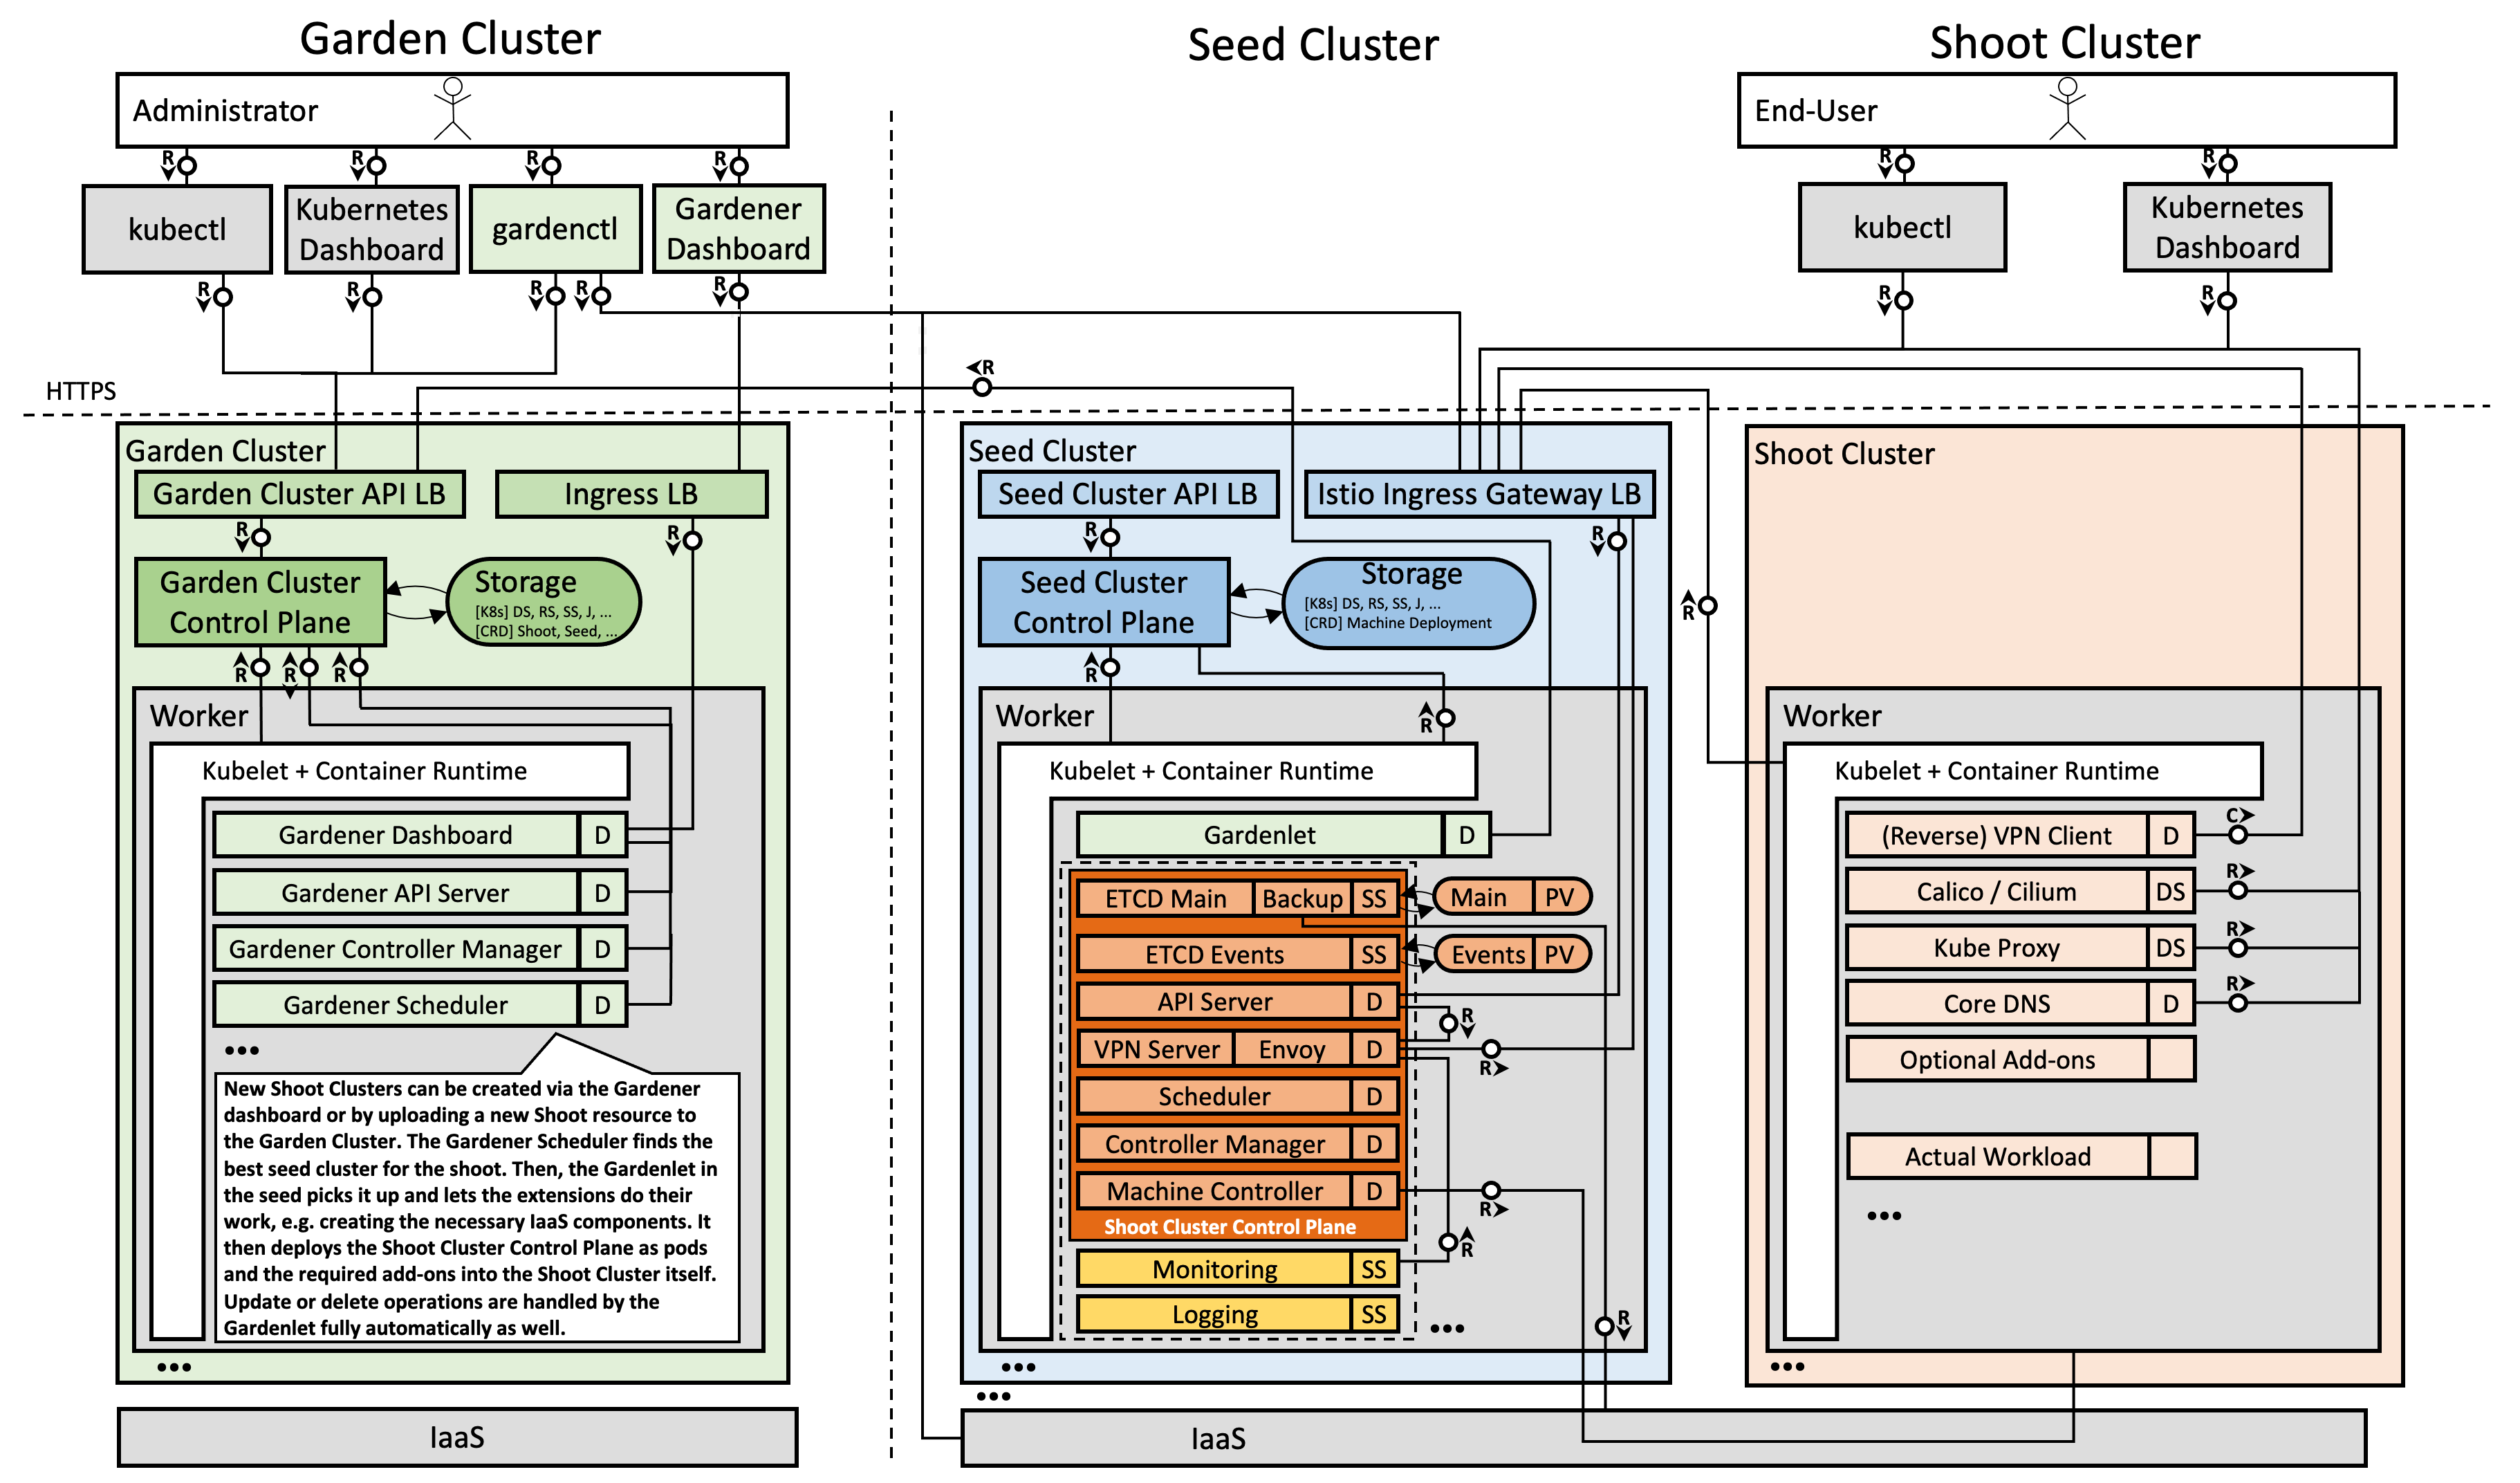
\includegraphics[width=\textwidth]{Bilder/gardener-architecture-detailed.png}
    \caption{Gardener architecture \cite{gardener.architecture}}
    \label{fig:gardener-architecture}
\end{figure}

% \begin{itemize}
%     \item open source software by SAP
%     \item for managing Kubernetes cluster (Kubernetes as a service)
%     \item Kubernetes native extension
    
%     \item cite https://kubernetes.io/blog/2018/05/17/gardener/
%     \item Even though there are tools that help with creating and updating single Kubernetes clusters, it is rather hard to manage many clusters.
%     \item there are tools to help in creating and updating single Kubernetes clusters
%     \item but very hard to manage many clusters
%     \item this is the focus of Gardener
%     \item manages Kubernetes clusters as a service
%     \item Gardener creates Kubernetes-conformant clusters
%     \item supports deployment to multiple cloud providers
%     \item brings the ability to manage thousands of clusters
%     \item 
% \end{itemize}

\section{\ac{aws}}
\acf{aws} is a subsidiary company of Amazon that offers a cloud computing platform with various services, such as \ac{s3} \cite{aws.s3} or \ac{eks} \cite{aws.eks}.
Started in 2006, \ac{aws} nowadays runs data centers all over the world to provide scalable, reliable, and high performing services. \cite{aws.linkedin, whatisaws}

At the time of writing, \ac{aws} is the cloud provider with the biggest market share. \cite{aws.marketshare}
Also, most of the supervising department's cloud service offerings are currently being deployed on \ac{aws}.
Because of these reasons and also due to constraints in time and complexity, the bootstrapping process worked out in this report is going to be narrowed down to deployment in an \ac{aws} environment.

\section{Terraform}
Modern enterprise infrastructure for software development usually makes use of cloud computing to dynamically adapt infrastructure to the fast-paced world of agile development.
These cloud services are usually distributed between multiple infrastructure providers, each of which uses their own individual \acp{api} to configure their platform.
Terraform is a tool that tries to minimize the effort needed to deploy these infrastructures in the long run by automating resource management as far as possible.
It allows to uniformly describe the target infrastructure in an easy to learn, machine-readable definition language and automatically takes care of deploying this infrastructure at the individual \ac{iaas} providers.
This approach is also known as \ac{iac}.
With Terraform, it is also possible to save provisioned infrastructure setups as a Terraform configuration to reuse them at a later point in time or to arbitrarily extend and adapt the configuration.
For configuration, either \ac{json} or \ac{hcl} can be used, with \ac{hcl} being the preferred way by the developing company HashiCorp because of its advanced features compared to \ac{json}.
Terraform can only unleash its full potential because of cooperations with all major software and hardware vendors and providers.
HashiCorp partners with over 160 companies and services the most noticeable ones being:
\begin{itemize}
    \item \ac{aws},
    \item Atlassian,
    \item Cloudflare,
    \item Google,
    \item Microsoft, and
    \item Oracle.
\end{itemize}

The most common use cases for Terraform include general \ac{iac}, managing Kubernetes (\autoref{sec:kubernetes}), multi-cloud deployment, management of network infrastructures, and management of virtual machine images.
Terraform additionally integrates tightly with other HashiCorp services like Vault (\autoref{sec:vault}).

% \begin{itemize}
%     \item codifies cloud apis into declarative configuration files
    
%     \item minimiert langfristig den für das Deploment benötigten Aufwand
%     \item um den modernen Ansprüchen der Schnelllebigkeit gerecht werden zu können, müssen IT-Administratoren Ressourcenmanagement weitmöglichst automatisieren
%     \item Kluster mit maschienenlesbaren Konfigurationscode beschreiben -> Infrastructure as Code
%     \item Terraform ermöglicht einheitliche Beschreibung von Zielinfrastruktur und sorgt für Umsetzung bei IaaS-Providern
%     \item erlaubt es, provisionierte Infrastruktur-Setups zu speichern, um diese zu einem späteren Zeitpunkt erneut nutzen oder beliebig erweitern/anpassen zu können
%     \item 160 Partner, sind unter anderem AWS, Atlassian, Cloudflare, Google, Microsoft und Oracle
    
%     \item üblicherweise wird auf verschiedene Cloud-Services zurückgegriffen um Infrastruktur für die Software-Entwicklung zu realisieren
%     \item daher menge verscheidedner Schnittstellen
%     \item mit Terraform aber nicht
%     \item statt individueller schnittstellensprache konfiguration über json oder HashiCorp Configurration Language (HCL)
%     \item hcl erlaubt kommentare und weitere features gegenüber json
    
%     \item Zusammenarbeit mit allen wichtigen Software und Hardware-Providern
    
%     \item häufige Anwendungsfälle für Terraform:
%     \item Infrastructure as Code
%     \item Multi-cloud deployment
%     \item Manage Kubernetes
%     \item Netzwerkinfrastruktur verwalten
%     \item Images von virtuellen Maschinen verwalten
%     \item Integration mit anderen HashiCorp Plattformen wie Vault
    
%     \item cite https://www.ionos.de/digitalguide/server/tools/was-ist-terraform/
%     \item cite https://www.terraform.io/
% \end{itemize}

\section{Jenkins}
Jenkins is a widely used open source automation server build with Java.
It is a \ac{cicd} tool aiming to save time by automating repetitive tasks like building projects, running test sets and deployment.
Jenkins supports many plugins (over 1800) via its update center which give you the ability to integrate with most of the common tools in development and automate practicably any project.
Jenkins can also be deployed on multiple machines to spread load and ensure quick and efficient operation.
\cite{jenkins.io, jenkins.github, gitlab.cicd}

In context of this project, Jenkins will be used after the successful bootstrap to take care of running Terraform and performing the actual deployment.

% \begin{itemize}
%     \item widely used open source automation server
%     \item built with Java
%     \item CICD tool (Continuous Integration and Continuous Delivery)
%     \item save time by automating repetitive tasks
%     \item like building projects, running tests and deployment
%     \item support for many plugins (over 1800) with its update center
%     \item give you the ability to deploy and automate any project
%     \item can be deployed on and spread load across multiple machines
%     \item cite https://www.jenkins.io/
%     \item cite https://github.com/jenkinsci/jenkins
    
%     \item 
% \end{itemize}

\section{Vault}
\label{sec:vault}
Vault is an open source service with the primary task to provide a central control unit to manage and organize enterprise secrets.
It encrypts secrets both at rest and in transit.
Access to the secrets can be granted granular per user through the use of \acp{acl}.
Furthermore, Vault audits access to the secrets.
That means that it keeps a detailed log on whom accessed what secret at which point in time.
If there was a security breach, where an unauthorized person got access to Vault, this protocol can be used to tell, if a specific secret has been read by the attacker or if it is still safe to use.

Vault is designed to be highly pluggable.
An instance is composed of \emph{storage backends}, \emph{audit log instances}, \emph{authentication providers} as well as \emph{secret backends}.
Each of these can be impersonated by a variety of different components.
This makes it possible to use different trusted authorities for attestation of identity.
For example, among others LDAP, JWT, GitHub, and Radius can be used.
An automated build service could very well use a different service to authenticate to Vault than a human user.

Secrets and encryption are often the weak spot in applications.
If a secret gets leaked and the leak stays unnoticed, attackers could gain long term access to a system.
As a solution, Vault offers \emph{dynamic secrets}.
When a client requests the access credentials for a supported system, Vault creates a short-lived secret just for that specific client.
Because the client is only accessing Vault, it does not have to bother with key creation nor rotation and an increased layer of security is added by not using secrets for an extended period of time.
Also, if a dynamic secret gets leaked, this single secret can be revoked individually.
If all clients accessing the resource used the same credentials, changing or blocking those could potentially cause an outage of the whole system.

When it comes to encryption, it can happen rather quickly that a single mistake compromises the security of the whole application.
Because of this, Vault offers encryption as a service.
The idea is, that Vault concentrates on the single task to handle credentials and encryption safely.
The broad variety of applications have a different focus and are not developed with the necessary expertise to guarantee safe implementation of security measures.
Vault, on the other hand, uses implementations that are audited by the open source community as well as independent experts.
Those are then provided as a high level \ac{api} to application developers.
That way, the encryption process of data gets very easy while, at the same time, Vault can handle the used encryption keys directly, and they are never actually sent to the application itself. \cite{vaultproject.io}

During the bootstrap, this project is about, a technical user is created for Terraform operations.
An access key is created for this user and then saved to Vault.
This way Jenkins then can obtain this access key and use it to perform the actual deployment with Terraform.

% \begin{itemize}
%     \item manage and organize secrets
%     \item provide a central secret storage
%     \item encrypt secrets at rest and in transit
%     \item ACL
%     \item Audit; log who has access what and when
%     \item a secret is a set of different credentials
%     \item protect sensitive data
%     \item various authentication methods; like LDAP, JWT, GitHub, Radius
%     \item authenticate against trusted sources of identity
%     \item trusted authority for attestation of identity
%     \item automate key issuance and rotation
    
%     \item dynamic secrets
%     \item create secrets for each specific client with limited lifetime
%     \item revoke a specific secret targeted
    
%     \item encrypt as a service
%     \item named key
%     \item high level API to do cryptography (encrypt, sign, verify, ...)
%     \item key and encryption logic never actually gets to the developer
%     \item control key lifecycle safely
%     \item protect application data at rest
    
%     \item highly pluggable
%     \item storage backends
%     \item Audit log instances
%     \item auth
%     \item secret backends (key/value, DB plugins, AWS, ...)
%     \item all of these are modular and can use solutions of various providers
    
%     \item cite https://www.vaultproject.io/
% \end{itemize}

\chapter{Future Work}
To finish off the bootstrap, work beyond the scope of this report is required.
Some fundamentals and considerations regarding these tasks shall be discussed here, although their realization will not be depicted.

\section{Establishing Tests for the Bootstrap}
When it comes to testing the implemented solution, it is important to distinguish different categories of tests.
On the one hand there are \emph{unit tests} and on the other there are \emph{integration tests}.

\paragraph{Unit tests} are about testing small components of code for functionality in different scenarios.
Do to so, the test often isolates the components from the remaining code.
Dependencies on other systems are usually swapped out to create this isolation.
This process is called \emph{mocking}.
In general, unit tests should not have side effects and should be completely independent of the rest of the application.
Because of this, unit tests are very fast, simpler in structure and therefore also easier to write.

\paragraph{Integration tests} on the other hand are way more complex than unit tests.
Like their name suggests, they test the integration of a module with other modules.
This is done when a unit test is not sufficient for testing some functions because of its isolation property.
Integration test do not try to mitigate side effects but consider them from the beginning.
Generally, integration tests are more complex to set up and slower than unit tests.
Also, integration test might often rely on external resources which failures are beyond the control of the developer.
As a result, it is usually desirable to use many unit tests and only few integration tests.

The difficulty with the implementation of the bootstrap at this state is that the interaction with \ac{aws} is deeply tied into the business logic of the bootstrap.
As a result, the bootstrap would require integration testing as a verification, although an integration test should only cover the actual interaction with \ac{aws} and not the bootstrap itself which should rather be checked with basic unit tests.
To cover the business logic of the bootstrap with unit tests, the bootstrap therefore has to be decoupled from the interaction with \ac{aws}.
The \ac{aws} part would then have to be covered with an integration test, although a much smaller one, which could focus solely on the third party service and would not get mixed with the departments own business logic.
To do so, there are different approaches that can be chosen from.

\paragraph{Client Interfaces} A common approach to write unit tests for something like the bootstrap would be to replace the clients of the \ac{aws} \ac{sdk} that communicate with the \ac{aws} backend with mocked clients.
These mocked clients could then fake the interaction with \ac{aws} and deliver reproducible results to test the actual business logic.
In Go, this is generally rather easy to achieve through the use of interfaces.
An interface in Go is just a definition of method headers.
Any type that implements the specified methods, automatically also implements the interface.
For making the actual clients interchangeable with mocked clients, interfaces would have to be specified, that define all \ac{sdk} methods the clients need.
Then, new types could be constructed, that implement those methods and return the desired values for mocking.
Now, instead of using the types of the actual \ac{sdk} clients when referring to the clients (in this case the types of the client variables in \autoref{code:aws-struct-1}), the interfaces would be used.
This enables the tests to replace the clients with the mocked clients without changing the program execution, because the same methods can be called but just on different objects.

This is an easy approach if only a few methods have to be mocked.
The problem in the context of this project is, that especially for the \ac{iam} client, many methods would have to be mocked individually, which is a lot of work, creates a lot of overhead for creating the interface, and it is difficult to cover all special cases and possible errors.

\paragraph{Function Pointers}
In some ways, this approach is rather similar to the aforementioned one.
In Go, functions can be stored in variables just like anything else.
So by extracting certain functionality into individual functions, instead of creating entire mock clients, just some functions could be swapped out for other functions delivering the mocked results.
To make use of this principle, another layer of abstraction would need to be implemented that wraps the \ac{sdk} methods into package scoped functions, and, if feasible, aggregates multiple \ac{sdk} methods into one wrapper.
These wrappers could be referred to with function pointers.
For unit testing, only these pointers would have to be adjusted to point to the mocked methods.
This can happen directly in the test file as in Go the tests are located in the same package.
The wrappers themselves could be verified for functionality with integration tests.

Although this approach reduces the complexity of the actual mocking by omitting the use of interfaces and rebuilding the entire clients, as a downside it would require some restructuring to the code because the calls to the \ac{sdk} methods would have to be replaced with the function pointers.

% \section{Integration with the \ac{cli}} % TODO: probably change number when more chapters arrive

% ---- Literaturverzeichnis
\cleardoublepage
\renewcommand*{\chapterpagestyle}{plain}
\pagestyle{plain}
\pagenumbering{Roman}                   % Römische Seitenzahlen
\setcounter{page}{\numexpr\value{savepage}+1}
\printbibliography[title=Literaturverzeichnis]

% ---- Anhang
\appendix
\include{Inhalt/04_Inhalt/1100_appendix}
%\clearpage
%\pagenumbering{Roman}  % römische Seitenzahlen für Anhang

\newpage
\end{document}
